\subsection*{7.6\hspace*{0.5cm}Impulses - Question}
Jen has a mass of 50kg and is in a car going $35\frac{m}{s}$ when she gets in an accident. The airbags deploy and bring her body to a stop in 0.500s. What is the force applied to her body?
\subsection*{7.6\hspace*{0.5cm}Impulses - Givens}
\begin{minipage}{0.5\textwidth}
    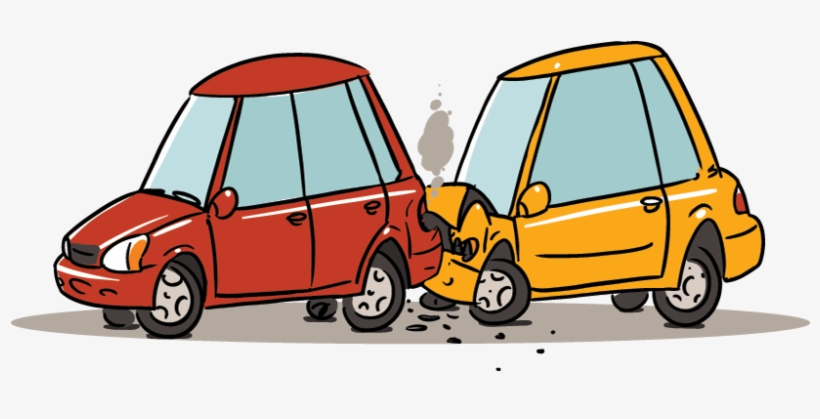
\includegraphics[scale=0.2]{./images/car_crash.png}
\end{minipage}
\begin{minipage}{0.5\textwidth}
    \begin{itemize}
        \item $v_{1} = 35\frac{m}{s}$
        \item $v_{2} = 0\frac{m}{s}$
        \item $\Delta t = 0.500s$
        \item $m_{J} = 50kg$
    \end{itemize}
\end{minipage}
\subsection*{7.6\hspace*{0.5cm}Impulses - Solve}
We can solve this problem using the equations provided in the Impulses section of this big book.\newline\newline
\textbf{1.} $\Delta P = F_{net}\Delta t$ \\
\begin{adjustwidth}{0.6cm}{0pt}
    $F_{net} = \frac{\Delta P}{\Delta t} = \frac{m\Delta v}{\Delta t} = \frac{m(v_{2} - v_{1})}{\Delta t}$ \\\\
    $\therefore F_{net} = \frac{50(0 - 35)}{0.500} \approx -3500N$
\end{adjustwidth}\vspace*{15pt}
\textbf{2.} $t = 0.100s$ \\
\begin{adjustwidth}{0.6cm}{0pt}
    $F_{net} = \frac{\Delta P}{\Delta t} = \frac{m\Delta v}{\Delta t} = \frac{m(v_{2} - v_{1})}{\Delta t}$ \\\\
    $\therefore F_{net} = \frac{50(0 - 35)}{0.100} \approx -17500N$
\end{adjustwidth}\vspace*{15pt}
\subsection*{7.6\hspace*{0.5cm}Impulses - Note}
Therefore if the time is lower, the less force the collision has on the person. This is why airbags are so important. Airbags reduce the time within the equation.
